%%%%%%%%%%%%%%%%%%%%%%%%%%%%%%%%%%%%%%%%%
% 2015SoE004
% SYSC Seminar Presentation
% Portland State University
% 16 October 2015
% %%%%%%%%%%%%%%%%%%%%%%%%%%%%%%%%%%%%%%%
% Presentation slides begin line 235
%----------------------------------------------------------------------------------------
%	PACKAGES AND OTHER DOCUMENT CONFIGURATIONS
%----------------------------------------------------------------------------------------

\documentclass[
paper=128mm:96mm, % The same paper size as used in the beamer class
fontsize=11pt, % Font size
pagesize, % Write page size to dvi or pdf
parskip=half-, % Paragraphs separated by half a line
]{scrartcl} % KOMA script (article)

\linespread{1.12} % Increase line spacing for readability

%------------------------------------------------
% Colors
\usepackage{xcolor}	 % Required for custom colors
% Define a few colors for making text stand out within the presentation
\definecolor{mygreen}{RGB}{44,85,17}
\definecolor{myblue}{RGB}{34,31,217}
\definecolor{mybrown}{RGB}{194,164,113}
\definecolor{myred}{RGB}{255,66,56}
% Use these colors within the presentation by enclosing text in the commands below
\newcommand*{\mygreen}[1]{\textcolor{mygreen}{#1}}
\newcommand*{\myblue}[1]{\textcolor{myblue}{#1}}
\newcommand*{\mybrown}[1]{\textcolor{mybrown}{#1}}
\newcommand*{\myred}[1]{\textcolor{myred}{#1}}
%------------------------------------------------

%------------------------------------------------
% Margins
\usepackage[ % Page margins settings
includeheadfoot,
top=3.5mm,
bottom=3.5mm,
left=5.5mm,
right=5.5mm,
headsep=6.5mm,
footskip=8.5mm
]{geometry}
%------------------------------------------------

%------------------------------------------------
% Fonts
\usepackage[T1]{fontenc}	 % For correct hyphenation and T1 encoding
\usepackage{lmodern} % Default font: latin modern font
%\usepackage{fourier} % Alternative font: utopia
%\usepackage{charter} % Alternative font: low-resolution roman font
\renewcommand{\familydefault}{\sfdefault} % Sans serif - this may need to be commented to see the alternative fonts
%------------------------------------------------

%-------------------------------------------------
%Graphics and figures organization
\usepackage{floatrow} 
\DeclareFloatSeparators{2 mm}
%\floatsetup[tmpset]{style=plain} -- a local setup

\usepackage{wrapfig} %L and R aligned images with captions and the text wrapped around 
                      %(how-to-text-wrap-an-image-in-latex)
%\usepackage{float} %fix position of figures w/ [H]; cannot use with \usepackage{floatrow}

%------------------------------------------------
% Presentation mode (uncomment for full screen)
%\usepackage{hyperref}
%\hypersetup{pdfpagemode=FullScreen}

%------------------------------------------------
% Various required packages
\usepackage{amsmath}
\usepackage{amsthm} % Required for theorem environments
\usepackage{bm} % Required for bold math symbols (used in the footer of the slides)
\usepackage{graphicx} % Required for including images in figures
\usepackage{tikz} % Required for colored boxes (I think this interferes w/ floatrow)
\usepackage{booktabs} % Required for horizontal rules in tables
\usepackage{multicol} % Required for creating multiple columns in slides
\setlength{\columnsep}{0.1mm}
\usepackage{lastpage} % For printing the total number of pages at the bottom of each slide
\usepackage[english]{babel} % Document language - required for customizing section titles
\usepackage{microtype} % Better typography
\usepackage{tocstyle} % Required for customizing the table of contents
\usepackage{caption}
\captionsetup{labelformat=empty,labelsep=none}
\usepackage{mathtools}
\usepackage{subcaption}
\usepackage{nicefrac}
%------------------------------------------------

%------------------------------------------------
% Slide layout configuration
\usepackage{scrpage2} % Required for customization of the header and footer
\pagestyle{scrheadings} % Activates the pagestyle from scrpage2 for custom headers and footers
\clearscrheadfoot % Remove the default header and footer
\setkomafont{pageheadfoot}{\normalfont\color{black}\sffamily} % Font settings for the header and footer

% Sets vertical centering of slide contents with increased space between paragraphs/lists
\makeatletter
\renewcommand*{\@textbottom}{\vskip \z@ \@plus 1fil}
\newcommand*{\@texttop}{\vskip \z@ \@plus .5fil}
\addtolength{\parskip}{\z@\@plus .25fil}
\makeatother

% Remove page numbers and the dots leading to them from the outline slide
\makeatletter
\newtocstyle[noonewithdot]{nodotnopagenumber}{\settocfeature{pagenumberbox}{\@gobble}}
\makeatother
\usetocstyle{nodotnopagenumber}

\AtBeginDocument{\renewcaptionname{english}{\contentsname}{\Large Outline}} % Change the name of the table of contents
%------------------------------------------------

%------------------------------------------------
% Header configuration - if you don't want a header remove this block
\ihead{
\hspace{-2mm}
\begin{tikzpicture}[remember picture,overlay]
\node [xshift=\paperwidth/2,yshift=-\headheight] (mybar) at (current page.north west)[rectangle,fill,inner sep=0pt,minimum width=\paperwidth,minimum height=2\headheight,top color=mygreen!64,bottom color=mygreen]{}; % Colored bar
\node[below of=mybar,yshift=3.3mm,rectangle,shade,inner sep=0pt,minimum width=128mm,minimum height =1.5mm,top color=black!50,bottom color=white]{}; % Shadow under the colored bar
shadow
\end{tikzpicture}
\color{white}\runninghead} % Header text defined by the \runninghead command below and colored white for contrast
%------------------------------------------------

%------------------------------------------------
% Footer configuration
%\newlength{\footheight}
\setlength{\footheight}{8mm} % Height of the footer
\addtokomafont{pagefoot}{\footnotesize} % Small font size for the footnote

\ifoot{% Left side
\hspace{-2mm}
\begin{tikzpicture}[remember picture,overlay]
\node [xshift=\paperwidth/2,yshift=\footheight] at (current page.south west)[rectangle,fill,inner sep=0pt,minimum width=\paperwidth,minimum height=3pt,top color=mygreen,bottom color=mygreen]{}; % Green bar
\end{tikzpicture}
\myauthor\ \raisebox{0.2mm}{$\bm{\vert}$}\ \myuni % Left side text
}

\ofoot[\pagemark/\pageref{LastPage}\hspace{-2mm}]{\pagemark/\pageref{LastPage}\hspace{-2mm}} % Right side
%------------------------------------------------

%------------------------------------------------
% Section spacing - deeper section titles are given less space due to lesser importance
\usepackage{titlesec} % Required for customizing section spacing
\titlespacing{\section}{0mm}{0mm}{0mm} % Lengths are: left, before, after
\titlespacing{\subsection}{0mm}{0mm}{-1mm} % Lengths are: left, before, after
\titlespacing{\subsubsection}{0mm}{0mm}{-2mm} % Lengths are: left, before, after
\setcounter{secnumdepth}{0} % How deep sections are numbered, set to no numbering by default - change to 1 for numbering sections, 2 for numbering sections and subsections, etc
%------------------------------------------------

%------------------------------------------------
% Theorem style
\newtheoremstyle{mythmstyle} % Defines a new theorem style used in this template
{0.5em} % Space above
{0.5em} % Space below
{} % Body font
{} % Indent amount
{\sffamily\bfseries} % Head font
{} % Punctuation after head
{\newline} % Space after head
{\thmname{#1}\ \thmnote{(#3)}} % Head spec
	
\theoremstyle{mythmstyle} % Change the default style of the theorem to the one defined above
\newtheorem{theorem}{Theorem}[section] % Label for theorems
\newtheorem{remark}[theorem]{Remark} % Label for remarks
\newtheorem{algorithm}[theorem]{Algorithm} % Label for algorithms
\makeatletter % Correct qed adjustment
%------------------------------------------------

%------------------------------------------------
% The code for the box which can be used to highlight an element of a slide (such as a theorem)
\newcommand*{\mybox}[2]{ % The box takes two arguments: width and content
\par\noindent
\begin{tikzpicture}[mynodestyle/.style={rectangle,draw=mygreen,thick,inner sep=2mm,text justified,top color=white,bottom color=white,above}]\node[mynodestyle,at={(0.5*#1+2mm+0.4pt,0)}]{ % Box formatting
\begin{minipage}[t]{#1}
#2
\end{minipage}
};
\end{tikzpicture}
\par\vspace{-1.3em}}
%------------------------------------------------
%----------------------------
%Specialty new commands
%arrow over vector
\newcommand{\amsvect}{%
  \mathpalette {\overarrow@\vectfill@}}
\def\vectfill@{\arrowfill@\relbar\relbar{\raisebox{-3.81pt}[\p@][\p@]{$\mathord\mathchar"017E$}}}
%----------------------------------------------------------------------------------------
%	PRESENTATION INFORMATION
%----------------------------------------------------------------------------------------
% Title
\newcommand*{\mytitle}{One Approach for Evaluating the Ecological Sustainability \\
of Agricultural Practices at the Landscape-scale}
% Running head displayed on almost all slides
\newcommand*{\runninghead}{Listening to the Landscape}
% Presenters name(s)
\newcommand*{\myauthor}{bmarron} 
% Presentation date
\newcommand*{\mydate}{16 October 2015} 
% University or department
\newcommand*{\myuni}{Portland State University} 

%----------------------------------------------------------------------------------------

\begin{document}

%----------------------------------------------------------------------------------------
%	INTRO SLIDES
%----------------------------------------------------------------------------------------
% title slide -----------------------------------------------------------------------------
\thispagestyle{empty} % No slide header and footer

\begin{tikzpicture}[remember picture,overlay] % Background box
%\node [xshift=\paperwidth/2,yshift=\paperheight/2] at (current page.south west)[rectangle,fill,inner
\node [xshift=\paperwidth/2,yshift=7 cm] at (current page.south west)[rectangle,fill,inner sep=0pt,minimum width=\paperwidth,minimum height=\paperheight/3,top color=mygreen,bottom color=mygreen]{};
\end{tikzpicture}
% Text within the box
\begin{flushright}
\vspace{-2.7cm}
\color{white}
\sffamily{\bfseries\normalsize\mytitle\par} % Title
\vspace{.1cm}
\normalsize
\myauthor\par % Author name
\vspace{-.3cm}
\mydate\par % Date
%\vfill
\end{flushright}
 \hspace*{2cm}
 \vspace*{-2cm}
 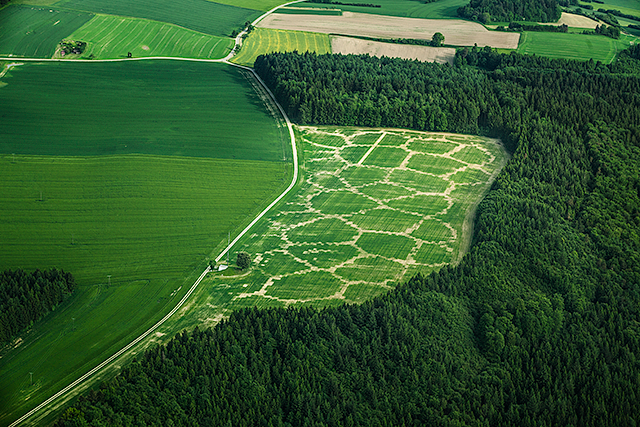
\includegraphics[height=1.0in]{Image1.png}
 \scriptsize {Avena+ Test Bed (created by Benedikt GroB)}

\clearpage
%----------------------------------------------------------------------------------------
%----------------------------------------------------------------------------------------
%	PRESENTATION SLIDES
%----------------------------------------------------------------------------------------
% slide ----------------------------------------------
\section{What we'll cover}


\normalsize
Personal motivations and bias\\
Some big questions and a few focused research questions\\
A very promising research approach\\
A novel methodology algorithm\\
Some exploratory results\\
Potential challenges and pitfalls\\
Next steps

\clearpage
%-------------------------------------------------------
% slide ----------------------------------------------
\section{Motivations and personal bias}
\begin{wrapfigure}{L}{0.3\textwidth}
\centering
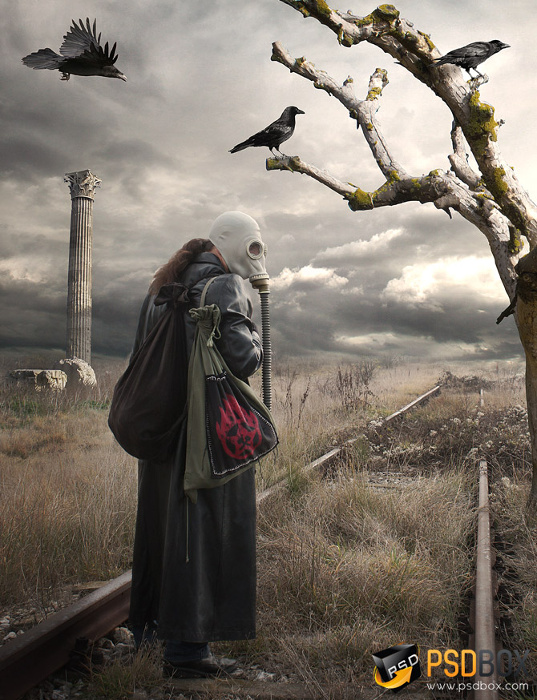
\includegraphics[height=0.95\textwidth]{Image2.jpg}
\caption{No, thanks.}
\end{wrapfigure}
\footnotesize 
\textasteriskcentered \ currently radiative forcing is about $1.5 \mathrm{Watts\textbackslash{m^2}}$\\
\textasteriskcentered \ currently we fix around $125 \ \mathrm{Tg N \textbackslash yr}$\\
\textasteriskcentered \ currently extinction rates are 10-1000x background\\

\clearpage
%-------------------------------------------------------
% slide ----------------------------------------------
\section{Motivations and personal bias}
\begin{wrapfigure}{L}{0.4\textwidth}
\centering
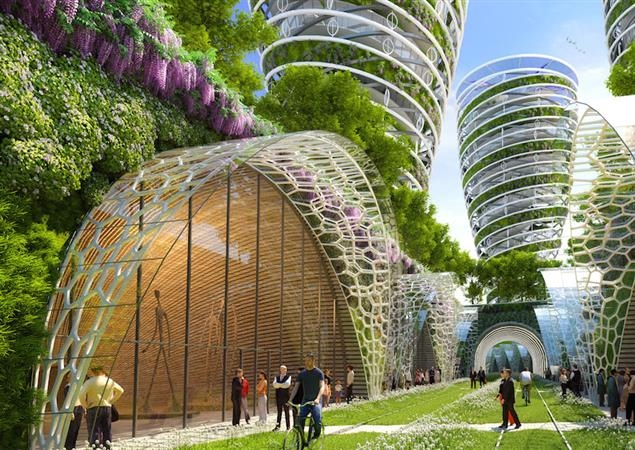
\includegraphics[width=0.85\textwidth]{Image3.jpg}
\caption{Yes, please!}
\end{wrapfigure}
\scriptsize
"Paris 2050 Project", Eco-utopian architect Vincent Callebaut\\

\clearpage
%-------------------------------------------------------
% slide ----------------------------------------------
\section{Motivations and personal bias}
\begin{wrapfigure}{L}{0.4\textwidth}
\centering
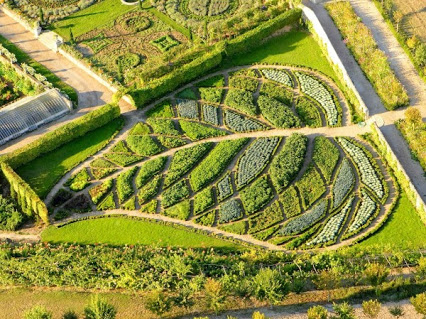
\includegraphics[width=0.85\textwidth]{Image4.jpg}
\caption{\scriptsize Maybe this but scaled up?}
\end{wrapfigure}
\scriptsize 
"The Garden of Abundance", Les Jardins de La Chatonniere, Ahmed Azeroual, Gardener-in-Chief
\clearpage
%-------------------------------------------------------
% slide ----------------------------------------------
\section{Motivations and personal bias}
\begin{wrapfigure}{L}{0.5\textwidth}
\scriptsize 
\centering
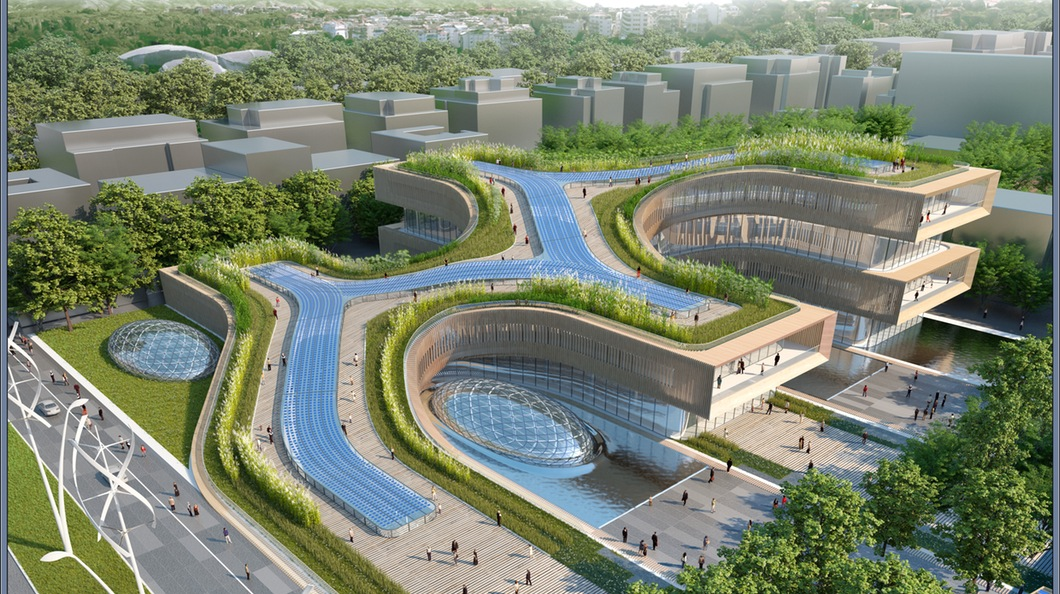
\includegraphics[width = 5 cm]{Image5.jpg}
\caption{\scriptsize  Rome's Eco-District, Vincent Callebaut}
\end{wrapfigure}
Food production systems that offer:\\
\textasteriskcentered \ minimal material and energetic inputs \\
\textasteriskcentered \ minimal externalized environmental \\
and social costs \\
\textasteriskcentered \ maximal nutritional output to People \\
and Planet\\
\textasteriskcentered \ maximal biodiversity

\clearpage
%-------------------------------------------------------
% slide ----------------------------------------------
\section{Motivations and personal bias}
\begin{wrapfigure}{L}{0.5\textwidth}
\scriptsize 
\centering
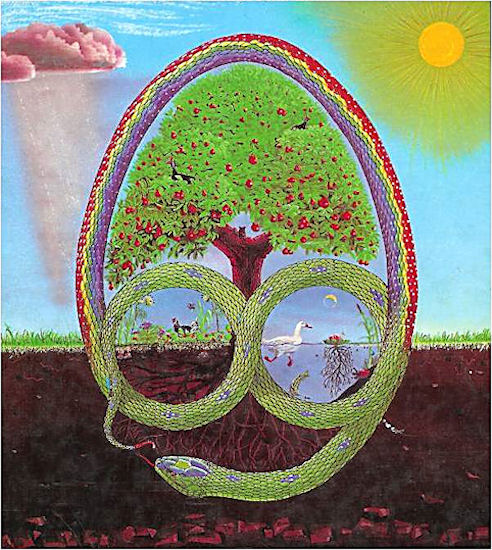
\includegraphics[height=3.5 cm]{Image19.jpg}
\caption{the egg of life}
\end{wrapfigure}
\textasteriskcentered care for the Earth\\
\textasteriskcentered care for the People \\
\textasteriskcentered take only what you need\\
\textasteriskcentered give back

\clearpage
%-------------------------------------------------------
% slide ----------------------------------------------
\subsection{Our end game}
\begin{wrapfigure}{L}{0.5\textwidth}
\scriptsize 
\centering
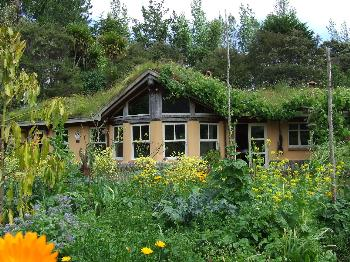
\includegraphics[height=3.5 cm]{Image20.jpg}
\caption{\tiny Rainbow Valley Farm, Matakana, NZ}
\end{wrapfigure}
Robust and adaptive food production systems designed at a regionally-specific, landscape scale (aka, 'sustainable agriculture')

\clearpage
%-------------------------------------------------------
% slide -----------------------------------------------
\subsection{But what does 'sustainable agriculture' actually mean?}
\small 
[see handout1, please]

\clearpage
%--------------------------------------------------------
% slide ----------------------------------------------
\section{A few of the big questions}
\footnotesize 
\textasteriskcentered \ Does a given food production system on a landscape enhance ecological resiliency or not?

%\textasteriskcentered \ What is the preferred configuration and practice of agriculture on any given landscape?

%\textasteriskcentered \ How can the dynamics of agro-ecological systems be used to develop dichotomous or synoptic keys for the classification of agricultural practices along the continuum of ecological resliency?

%\textasteriskcentered \ What suite of pattern recognition tools can be used to logically, and ultimately causally, link ecological processes to landscape-scale patterns?
\clearpage
%-------------------------------------------------------
% slide ----------------------------------------------
\section{A few of the big questions}
\footnotesize 
\textasteriskcentered \ Does a given food production system on a landscape enhance ecological resiliency or not?

\textasteriskcentered \ What is the preferred configuration and practice of agriculture on any given landscape?

%\textasteriskcentered \ How can the dynamics of agro-ecological systems be used to develop dichotomous or synoptic keys for the classification of agricultural practices along the continuum of ecological resliency?

%\textasteriskcentered \ What suite of pattern recognition tools can be used to logically, and ultimately causally, link ecological processes to landscape-scale patterns?
\clearpage
%-------------------------------------------------------
% slide ----------------------------------------------
\section{A few of the big questions}
\footnotesize 
\textasteriskcentered \ Does a given food production system on a landscape enhance ecological resiliency or not?

\textasteriskcentered \ What is the preferred configuration and practice of agriculture on any given landscape?

\textasteriskcentered \ How can the dynamics of agro-ecological systems be used to develop dichotomous or synoptic keys for the classification of agricultural practices along the continuum of ecological resliency?

%\textasteriskcentered \ What suite of pattern recognition tools can be used to logically, and ultimately causally, link ecological processes to landscape-scale patterns?
\clearpage
%-------------------------------------------------------
% slide ----------------------------------------------
\section{A few of the big questions}
\footnotesize 
\textasteriskcentered \ Does a given food production system on a landscape enhance or reduce ecological resiliency?

\textasteriskcentered \ What is the preferred configuration and practice of agriculture on any given landscape?

\textasteriskcentered \ How can the dynamics of agro-ecological systems be used to develop dichotomous or synoptic keys for the classification of agricultural practices along the continuum of ecological resiliency?

\textasteriskcentered \ What suite of pattern recognition tools can be used to logically, and ultimately causally, link ecological processes to landscape-scale patterns?
\clearpage
%-------------------------------------------------------
% slide ----------------------------------------------
\section{Important research questions for me}
\scriptsize 
\textasteriskcentered \ What is the relationship between landscape-scale disturbance regimes, agricultural output, and biodiversity? Which landscape mosaic is the 'most appropriate' one to maintain?

%\textasteriskcentered \ What is the n-dimensional vector of state variables from agro-ecological systems that is necessary and sufficient to assess the current ecological health and resiliency of a given landscape pattern and to evaluate the ecological health and resiliency of simulated landscape patterns (scenarios)?

%\textasteriskcentered \ Can a modeling environment be created that captures the spatial and temporal evolution of those critical ecological and environmental processes which are, in large measure, responsible for the patterned heterogeneity of an agro-ecological landscape?

%\textasteriskcentered \ What are the critical elements and processes shared by historical examples of both successful and disastrous agroecological practices that can inform our transition to sustainable agriculture?
\clearpage
%-------------------------------------------------------
% slide ----------------------------------------------
\section{Important research questions for me}
\textasteriskcentered \ What is the relationship between landscape-scale disturbance regimes, agricultural output, and biodiversity? Which landscape mosaic is the 'most appropriate' one to maintain?

\textasteriskcentered \ What is the n-dimensional vector of state variables from agro-ecological systems that is necessary and sufficient to assess the current ecological health and resiliency of a given landscape pattern and to evaluate the ecological health and resiliency of simulated landscape patterns (scenarios)?

%\textasteriskcentered \ Can a modeling environment be created that captures the spatial and temporal evolution of those critical ecological and environmental processes which are, in large measure, responsible for the patterned heterogeneity of an agro-ecological landscape?

%\textasteriskcentered \ What are the critical elements and processes shared by historical examples of both successful and disasterous agroecological practices that can inform our transition to sustainable agriculture?
\clearpage
%-------------------------------------------------------
% slide ----------------------------------------------
\section{Important research questions for me}
\textasteriskcentered \ What is the relationship between landscape-scale disturbance regimes, agricultural output, and biodiversity? Which landscape mosaic is the 'most appropriate' one to maintain?

\textasteriskcentered \ What is the n-dimensional vector of state variables from agro-ecological systems that is necessary and sufficient to assess the current ecological health and resiliency of a given landscape pattern and to evaluate the ecological health and resiliency of simulated landscape patterns (scenarios)?

\textasteriskcentered \ Can a modeling environment be created that captures the spatial and temporal evolution of those critical ecological and environmental processes which are, in large measure, responsible for the patterned heterogeneity of an agro-ecological landscape?

%\textasteriskcentered \ What are the critical elements and processes shared by historical examples of both successful and disasterous agroecological practices that can inform our transition to sustainable agriculture?
\clearpage
%-------------------------------------------------------
% slide ----------------------------------------------
\section{Important research questions for me}
\textasteriskcentered \ What is the relationship between landscape-scale disturbance regimes, agricultural output, and biodiversity? Which landscape mosaic is the 'most appropriate' one to maintain?

\textasteriskcentered \ What is the n-dimensional vector of state variables from agro-ecological systems that is necessary and sufficient to assess the current ecological health and resiliency of a given landscape pattern and to evaluate the ecological health and resiliency of simulated landscape patterns (scenarios)?

\textasteriskcentered \ Can a modeling environment be created that captures the spatial and temporal evolution of those critical ecological and environmental processes which are, in large measure, responsible for the patterned heterogeneity of an agro-ecological landscape?

\textasteriskcentered \ What are the critical elements and processes shared by historical examples of both successful and disasterous agroecological practices that can inform our transition to sustainable agriculture?
\clearpage
%-------------------------------------------------------
% slide ----------------------------------------------
%Image7 is from PRF002
\section {A very promising research approach}
\scriptsize
\begin{minipage}{.4\textwidth}
   \centering
  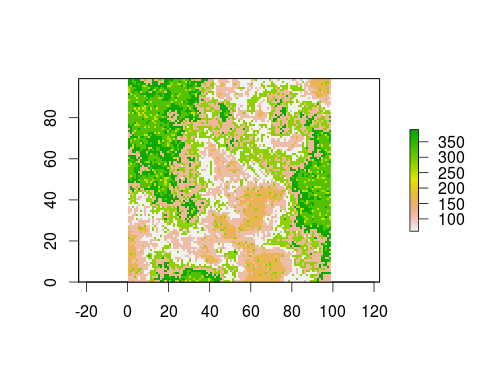
\includegraphics[width=.8\linewidth]{Image6}
  \captionof{figure}{LANDIS-II}
 \end{minipage}
+
\begin{minipage}{.4\textwidth}
  \centering
  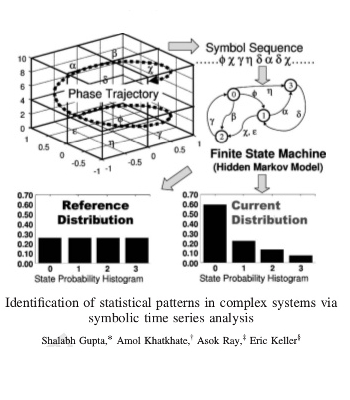
\includegraphics[width=.8\linewidth]{Image7}
  \captionof{figure}{Symbolic Dynamics}
\end{minipage}

\clearpage
%-------------------------------------------------------
% slide ----------------------------------------------
\section{Why this approach?}
\normalsize 
[see handout2, please]
\clearpage
%-------------------------------------------------------
% slide ----------------------------------------------
\section{Why this approach?}
\centering 
\includegraphics[height=5.75 cm]{Image21.jpg}
\clearpage
%-------------------------------------------------------
% slide ----------------------------------------------
\section{Why this approach?}
\centering 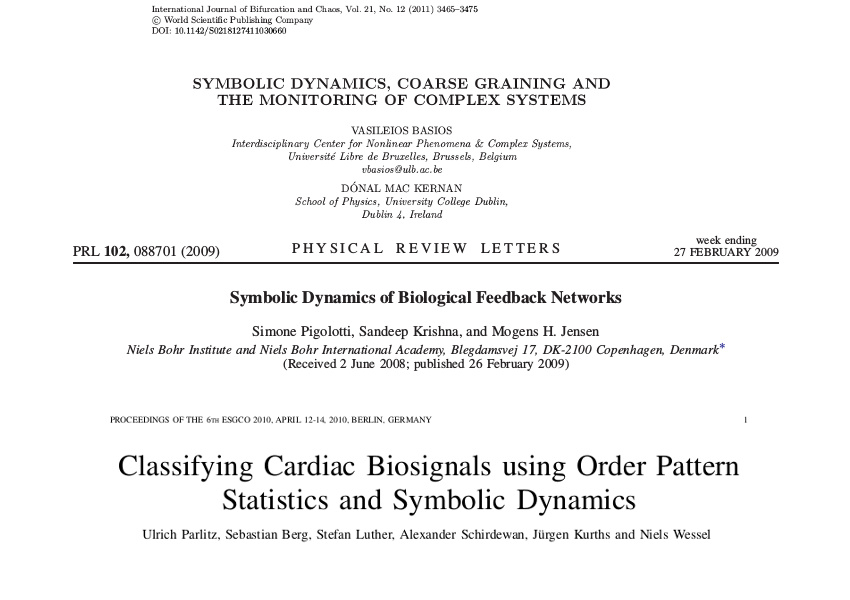
\includegraphics[height=5.5 cm]{Image22.jpg}
\clearpage
%-------------------------------------------------------
% slide ----------------------------------------------
\section{Why this approach?}

\begin{flushleft}
Here's what Claire says,\\
"We are creating spatially explicit models based on resource availability, resource needs, and foraging scales, to develop alternative scenarios for managing the agro-natural landscape for pollination function."
\end{flushleft}
\begin{flushright}
-- Claire Kremen, Department of Ecology \\
and Evolutionary Biology, Princeton
\begin{verbatim}
[Ecology Letters, (2005) 8: 468-479]
\end{verbatim}
\end{flushright}

\clearpage
%-------------------------------------------------------
% slide ----------------------------------------------
\section{The proposed algorithm}
\subsection{Level I: Build an m-dimensional vector of state variables.}
\subsection{Level II: Define a set of landscape reference scenarios.}
\subsection{Level III: Translate the landscape reference scenarios to LANDIS-II.}
\subsection{Level IV: Build a landscape reference scenario codebook.}
\clearpage
%-------------------------------------------------------
% slide ----------------------------------------------
\section{The proposed algorithm}
\subsection{Level V: Build m-order Markov chains (bigram models) for the reference landscape scenarios.}
\subsection{Level VI: Define agro-ecological sustainability for a given landscape.}
\subsection{Level VII: Evaluate the sustainability vocabulary of extant and novel landscape designs.}
\clearpage
%-------------------------------------------------------
% slide ----------------------------------------------
\section{The proposed algorithm}
\subsection{Level I: Build an m-dimensional vector of state variables.}
\[ \amsvect{KMVV} = (kmv_{1}, kmv_{2}, kmv_{3}, kmv_{4}, kmv_{5}, ... kmv_{m})\]

\clearpage
%-------------------------------------------------------
% slide ------------------------------------------------
\begin{figure}[h]
\centering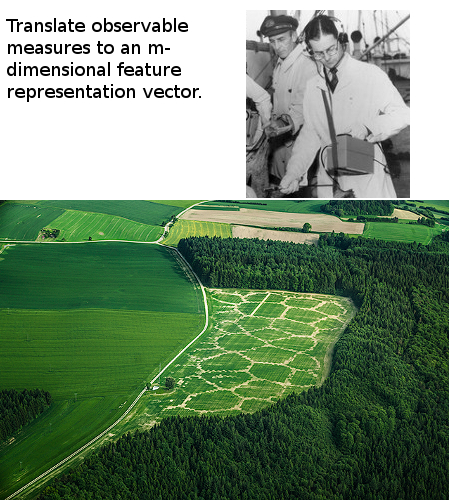
\includegraphics[height=0.6\linewidth]{Image8.jpg}
\end{figure}

\clearpage
%-------------------------------------------------------
% slide ----------------------------------------------
\subsection{Level I: Build an m-dimensional vector of state variables.}
\small
\begin{tabular}{lll}
  \textbf{Step 1} & ==> & Select the set of key monitoring variables (KMVs) for\\
  & & agro-ecosystems at the landscape scale
\end{tabular}

\textbf{Many choices!}\\
\begin{flushleft}
 [see handout1, please]
 \end{flushleft} 
\clearpage
%-------------------------------------------------------
% slide ----------------------------------------------
\subsection{Level I: Build an m-dimensional vector of state variables.}
\begin{tabular}{lll}
  \textbf{Step 2} & ==> & Fix the n-dimensional vector of required empirical variables \\
  & & (the REVV)\\
  & ==> & Automate the calculation of the m-dimensional vector of key \\
  & & monitoring variables (the KMVV)
\end{tabular}

\clearpage
%-------------------------------------------------------
% slide ----------------------------------------------
\section{The proposed algorithm}
\subsection{Level II: Define a set of landscape reference scenarios.}
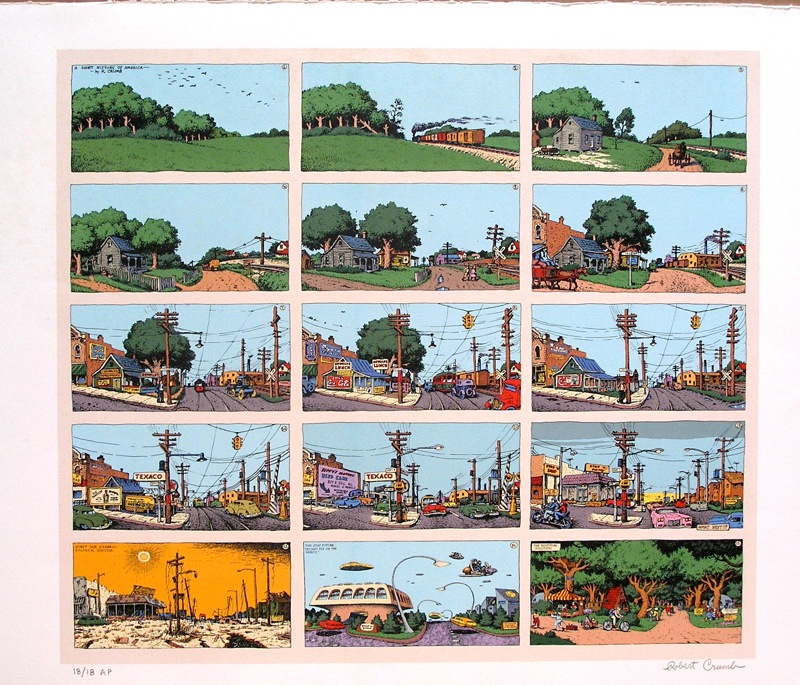
\includegraphics[height=5 cm]{Image13.jpg}
\footnotesize R. Crumb

\clearpage
%-------------------------------------------------------
% slide ----------------------------------------------
\subsection{Level II: Define a set of landscape reference scenarios.}
\begin{tabular}{lll}
\textbf{Step 3a} & ==> &Define five reference systems of human impact and presence\\
& &on the landscape (so-called HIP classes)\\
& ==> & HIP classes A through E are defined by \% agriculture, \\
& &\% forest, and \% built environment on the landscape\\
& ==> & HIP subclasses are defined by unique definitions of agri-\\
& & culture, forest, and built environment
\end{tabular} 

\clearpage
%-------------------------------------------------------
% slide ------------------------------------------------
\subsection{Level II: Define a set of landscape reference scenarios.}
\begin{table}[h]
\footnotesize 
\centering
\begin{tabular}{l l l l}
\toprule
\textbf{HIP Class} & \textbf{\% Ag.} & \textbf{\% Forest} & \textbf{\% Built Env.}\\
\midrule
A & 5.0 & 90.0 & 5.0 \\
B & 20.0 & 75.0 & 5.0 \\
C & 40.0 & 50.0 & 10.0 \\
D & 80.0 & 5.0 & 15.0 \\
E & 5.0 & 5.0 & 90.0 \\
\bottomrule
\end{tabular}
\caption{\scriptsize Five reference systems of human impact and presence (HIP) on the landscape.}
\end{table}

\clearpage
%------------------------------------------------------
% slide ----------------------------------------------
\subsection{Level II: Define a set of landscape reference scenarios.}
\begin{tabular}{lll}
	\textbf{Step 3b} & ==> & Define 'agriculture', 'forest', and 'built environment' for \\
	& & HIP subclass1
\end{tabular} 

\begin{tabular}{lll}
  Agriculture & == &intensely managed land using standard, \underline{\textit{agribusiness}}\\
  & & \underline{\textit{practices}}\\
 Forest & == &lightly-managed land covered in locally-appropriate\\
 & & vegetation\\
 Built environment & == &land completely unavailable for photosynthetic\\
 & & activity (zero net primary productivity)
\end{tabular}

\clearpage
%-------------------------------------------------------
% slide ----------------------------------------------
\subsection{Level II: Define a set of landscape reference scenarios.} 
\begin{tabular}{lll}
	\textbf{Step 3c} & ==> & Define 'agriculture', 'forest', and 'built environment' for \\
	& & HIP subclass2
\end{tabular} 

\begin{tabular}{lll}
  Agriculture & == &intensely managed land using \underline{\textit{agro-ecological}}\\
  & & \underline{\textit{practices}}\\
 Forest & == &lightly-managed land covered in locally-appropriate\\
 & & vegetation\\
 Built environment & == &land completely unavailable for photosynthetic\\
 & & activity (zero net primary productivity)
\end{tabular}

\clearpage
%-------------------------------------------------------
% slide ----------------------------------------------
\section{The proposed algorithm}
\subsection{Level III: Translate the landscape reference scenarios to LANDIS-II.}
\ffigbox{
        {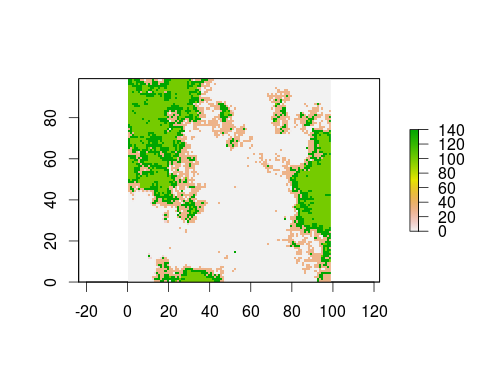
\includegraphics[width=.4\linewidth]{Image14.png}}
        {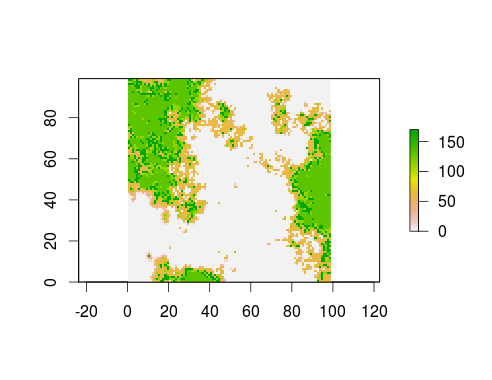
\includegraphics[width=.4\linewidth]{Image16.png}}
        {$\xrightarrow{Time}$}
    }
    
\clearpage
%-------------------------------------------------------
% slide ------------------------------------------------
\subsection{Level III: Translate the landscape reference scenarios to LANDIS-II.}
\footnotesize 
\begin{tabular}{lll}
	\textbf{Step 4a} & ==> & Define the set of landscape patches for each of the\\
	& & reference systems defined by an HIP subclass\\
\end{tabular}

\[ HIP \ subclasses = \{ A1, B1, C1, D1, E1, A2, B2, C2, D2, E2\} \]
\clearpage
%-------------------------------------------------------
% slide ------------------------------------------------
\subsection{Level III: Translate the landscape reference scenarios to LANDIS-II.}
\begin{tabular}{lll}
	\textbf{Step 4b} & ==> & Provide each patch-type with a unique moniker, a unique \\
	& & MapCode, a spp. list, and spp. age distribution for building \\
	& & LANDIS-II 'initial communities' files
\end{tabular}
\tiny 
\begin{verbatim}
LandisData   "Initial Communities"
>>Old jackpine oak 
MapCode  0
   acerrubr 30
   pinubank 80 90
   pinuresi 110 140
   querelli 40 120 240
>> young jackpine oak
MapCode  1
   pinubank 30 50
   querelli 10 40 70
\end{verbatim}

\clearpage
%------------------------------------------------------
% slide ------------------------------------------------
\subsection{Level III: Translate the landscape reference scenarios to LANDIS-II.}
\ffigbox{
        {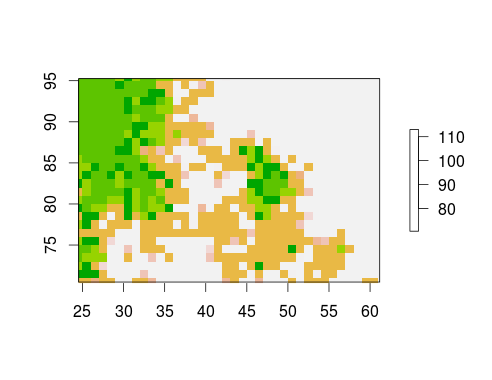
\includegraphics[height=4 cm]{Image17.png}}
        }    
    \tiny 
 \begin{verbatim}
 initialCommunities[1,]
 [1] 5 5 6 5 5 5 4 4 3 4 4 4 5 4 4 3 3 4 5 5 5 6 6 6 6 6 6 6 6 6 5 4 3 4 4 4 5
[38] 5 5 4 4 4 2 2 1 1 1 1 1 2 2 1 1 1 2 2 2 2 2 2 1 1 3 2 2 2 2 2 2 3 2 2 2 1
[75] 2 2 2 2 2 2 0 1 2 2 1 2 2 2 1 1 0 0 0 0 0 0 0 0 0
 \end{verbatim}   

\clearpage
%---------------------------------------------------------
\subsection{Level III: Translate the landscape reference scenarios to LANDIS-II.}
\footnotesize 
\begin{tabular}{lll}
	\textbf{Step 5} & ==> & Operationalize the LANDIS-II model for each\\
	& & of the HIP subclass reference systems\\
	& ==> & "Operationalize" means to parameterize, calibrate (validate), \\
	& & and define the simulation settings for each model
\end{tabular}

\clearpage
% slide ----------------------------------------------
\section{The proposed algorithm}
\subsection{Level IV: Build a landscape reference scenario codebook.}
\ffigbox{
        {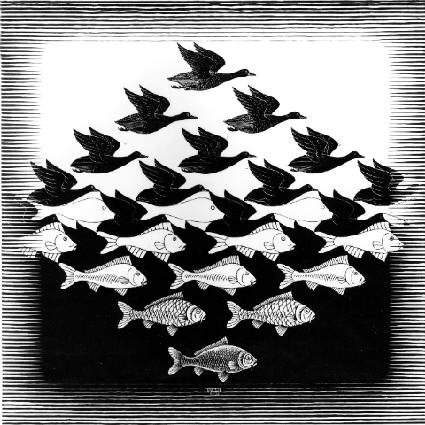
\includegraphics[height=.3\linewidth]{Image18.jpg}}
        = \{aabbcdddd\}\\
        MC Escher
    }
    
\clearpage
%-------------------------------------------------------
% slide ------------------------------------------------
\subsection{Level IV: Build a landscape reference scenario codebook.}
\footnotesize 
\begin{tabular}{lll}
	\textbf{Step 6} & ==> & Perform multiple simulation runs (min r=3) \\
	& & for each of the HIP subclasses\\
	& ==> & Each dataset is a time series (t = 20) of the n-dimensional REVV; \\
	& & $\sim$ 30 data sets generated\\
	& ==> & Transform all raw output data (i.e., all REVVs) to KMVVs\\
	& & keeping time stamps intact
\end{tabular}

\clearpage
%-------------------------------------------------------
% slide ------------------------------------------------
\subsection{Level IV: Build a landscape reference scenario codebook.}
\footnotesize 
\begin{tabular}{lll}
	\textbf{Step 7} & ==> & Define a set of unique landscape morphs (states)\\
	& & for each landscape reference scenario\\
	& ==> & Morphs are derived from the collection of KMVVs\\
	& & generated by LANDIS-II using a feature extraction method
\end{tabular}

\clearpage
%-------------------------------------------------------
% slide ------------------------------------------------
\textbf{\normalsize Many methods for identifying unique landscape morphs.\\
Choose one or more.}
\begin{flushleft}
Hidden Markov Model?\\
Multi-section Vector Quantizer?\\
Support Vector Machine?\\
k-means Non-hierarchical Clustering Algorithm?\\
Principal Components Analysis?\\
Hierarchical Neural Network?\\
Logistic Regression?\\
Discriminant Analysis?
\end{flushleft}

\clearpage
%-------------------------------------------------------
% slide ------------------------------------------------
\textbf{\normalsize And many measures can be used by the methods!\\
Choose one or more.}
\begin{flushleft}
Information measures\\ 
Distance measures\\
Dependence measures\\
Consistency measures\\
Accuracy measures
\end{flushleft}

\clearpage
%-------------------------------------------------------
% slide ------------------------------------------------
\subsection{Level IV: Build a landscape reference scenario codebook.}
\footnotesize 
\begin{tabular}{lll}
	\textbf{Step 8a} & ==> & Codify the morphs generated by each landscape reference scenario \\
	& & by giving each one a unique character symbol\\
	& ==> & Compile the symbols, their prototype (reproduction) KMVVs,  \\
	& & and their probability distributions into a codebook\\
	& ==> & A "codebook" is a collection of symbols, prototype (reproduction)\\
	& &  KMVVs, and probability distributions
	
\end{tabular}

\clearpage
%-------------------------------------------------------
% slide ------------------------------------------------
\subsection{Level IV: Build a landscape reference scenario codebook.}
\footnotesize 
\begin{tabular}{lll}
	\textbf{Step 8b} & ==> & Combine the five codebooks generated by HIP subclass1\\
	& & into one codebook, Alphabet1\\
	& ==> & Combine the five codebooks generated by HIP subclass2\\
	& & into one codebook, Alphabet2
\end{tabular}

\clearpage
%-------------------------------------------------------
% slide ------------------------------------------------
\subsection{Level IV: Build a landscape reference scenario codebook.}
\footnotesize 
\begin{tabular}{lll}
	\textbf{Step 8c} & ==> & Define the complete landscape reference scenario codebook as\\
	& & the collection of Alphabet1 plus Alphabet2
\end{tabular}

\clearpage
%-------------------------------------------------------
% slide ----------------------------------------------
\section{The proposed algorithm}
\subsection{Level V: Build m-order Markov chains (bigram models) for the reference landscape scenarios.}
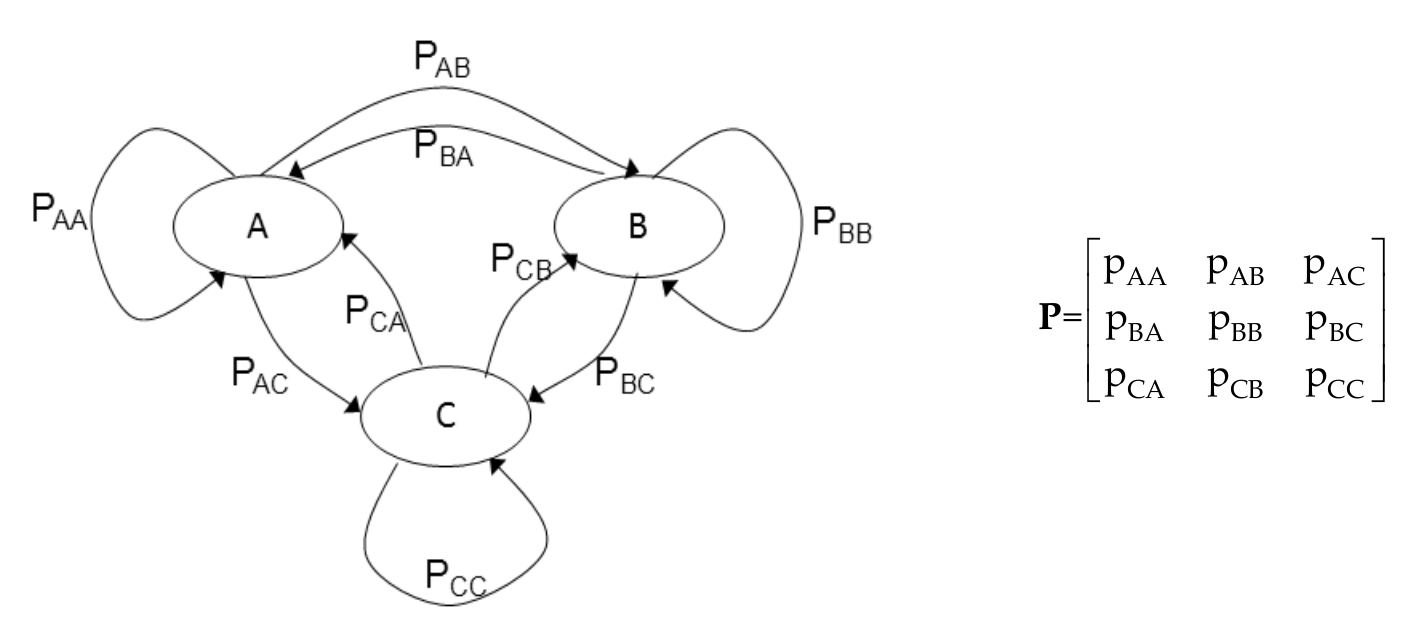
\includegraphics[height=3 cm]{Image23.jpg}\\
\footnotesize Time series data for 3 morphs on the landscape = {AABBBABCBBBCBAA...}
\clearpage
%-------------------------------------------------------
% slide ------------------------------------------------
\subsection{Level V: Build m-order Markov chains (bigram models) for the reference landscape scenarios.}
\footnotesize 
\begin{tabular}{lll}
	\textbf{Step 9} & ==> & Apply the landscape reference scenario codebook to the \\
	& & original KMVV data set to obtain landscape morph time series \\
	& &  data (sequences of symbols) for each reference scenario\\
	& ==> & This process will generate 10 sets of symbolic data
	
\end{tabular}

\clearpage
%-------------------------------------------------------
% slide ------------------------------------------------
\subsection{Level V: Build m-order Markov chains (bigram models) for the reference landscape scenarios.}
\footnotesize 
\begin{tabular}{lll}
	\textbf{Step 10a} & ==> & Extract empirical frequencies from the time series data \\
	& & and use them to derive 1-step conditional probabilities 	
\end{tabular}
\begin{align*}
Logical \ product \ rule \ (Bayes)\\
p(AB) \ &= \ p(A|B)p(B) \ = \ p(B|A)p(A)\\
p(A|B) \ &= \ \nicefrac{p(AB)}{p(B)}\\
p(B|A) \ &= \ \nicefrac{p(AB)}{p(A)}
\end{align*}


\clearpage
%-------------------------------------------------------
% slide ------------------------------------------------
\subsection{Level V: Build m-order Markov chains (bigram models) for the reference landscape scenarios.}
\footnotesize 
\begin{tabular}{lll}
	\textbf{Step 10b} & ==> & Define a bigram model from the conditional probabilities \\
\end{tabular}
\begin{equation*}
\begin{aligned}
Transition \ (stochastic) \ matrix\\
p(A|A) \ &= .25\\
p(B|A) \ &= .75\\
p(A|B) \ &= .10\\
p(B|B) \ &= .90
\end{aligned}
=
\begin{aligned}
\begin{bmatrix}
	.25_{A|A} & .75_{B|A}\\
	.10_{A|B} & .90_{B|B}
\end{bmatrix}
\end{aligned}
\end{equation*}

\clearpage
%-------------------------------------------------------
% slide ----------------------------------------------
\section{The proposed algorithm}
\subsection{Level VI: Define agro-ecological sustainability for a given landscape.}
\begin{equation*}
\begin{aligned}
Landscape \ morphs\\
A \ &= morph_{1}\\
B \ &= morph_{2}\\
C \ &= morph_{3}\\
...\\
A \ landscape \ sustainability \ shift \ space\\
\big[ A\geq  pr_{1}, \ B\leq pr_{2}, \ pr_{3}\leq C \leq pr_{4}, \ ... \big]
\end{aligned}
\end{equation*}

\clearpage
%-------------------------------------------------------
% slide ------------------------------------------------
\subsection{Level VI: Define agro-ecological sustainability for a given landscape.}
\footnotesize 
\begin{tabular}{lll}
	\textbf{Step 11} & ==> & Evaluate the ecological implications of the correlations \\
	& & evident in the transition (stochastic) matrices
\end{tabular}

\begin{equation*}
\begin{aligned}
\begin{bmatrix}
	.50_{A|A} & .50_{B|A}\\
	.50_{A|B} & .50_{B|B}
\end{bmatrix}\\
\end{aligned}
vs.
\begin{aligned}
\begin{bmatrix}
	.75_{A|A} & .25_{B|A}\\
	.95_{A|B} & .05_{B|B}
\end{bmatrix}\\
\end{aligned}
\end{equation*}
\begin{equation*}
\begin{aligned}
\begin{bmatrix}
	1_{A|A} & 0_{B|A}\\
	0_{A|B} & 1_{B|B}
\end{bmatrix}\\
\end{aligned}
vs.
\begin{aligned}
\begin{bmatrix}
	0_{A|A} & 1_{B|A}\\
	1_{A|B} & 0_{B|B}
\end{bmatrix}\\
\end{aligned}
\end{equation*}

\clearpage
%-------------------------------------------------------
% slide ------------------------------------------------
\subsection{Level VI: Define agro-ecological sustainability for a given landscape.}
\footnotesize 
\begin{tabular}{lll}
	\textbf{Step 12} & ==> & Use ecological and biological principles to evaluate agro-ecological\\
	& & sustainability by examining the fluxes in the components of the \\
	& & KMVV relative to the sequence of morphs appearing over time
\end{tabular}
\begin{flushleft}
Are the arbuscular mycorrhizal fungi increasing? Decreasing? Holding steady?
\end{flushleft}
\clearpage
%-------------------------------------------------------
% slide ------------------------------------------------
\subsection{Level VI: Define agro-ecological sustainability for a given landscape.}
\footnotesize 
\begin{tabular}{lll}
	\textbf{Step 13} & ==> & Ideally, we would be able to evaluate agro-ecological \\ 
	& & sustainability on a given landscape by defining a shift space where \\
	& & the "forbidden blocks" are thresholds in the stationary distribution \\
	& & of landscape morphs
\end{tabular}
\begin{equation*}
\big[ A\geq  pr_{1}, \ B\leq pr_{2}, \ pr_{3}\leq C \leq pr_{4}, \ ... \big]
\end{equation*}
\clearpage
%-------------------------------------------------------
% slide ----------------------------------------------
\section{The proposed algorithm}
\subsection{Level VII: Explore the sustainability vocabulary of extant and novel landscape designs.}
\centering 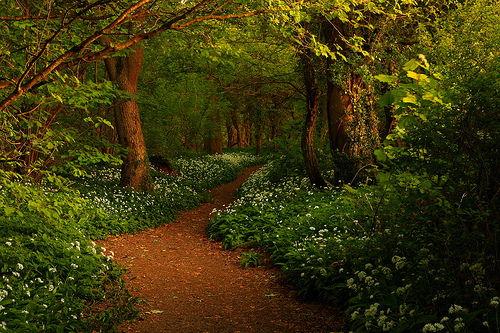
\includegraphics[height=4 cm]{Image24.jpg}\\
a food forest
\clearpage
%-------------------------------------------------------
% slide ----------------------------------------------
\section{By golly, it just might work!}
\subsection{Some experimental results}
\centering 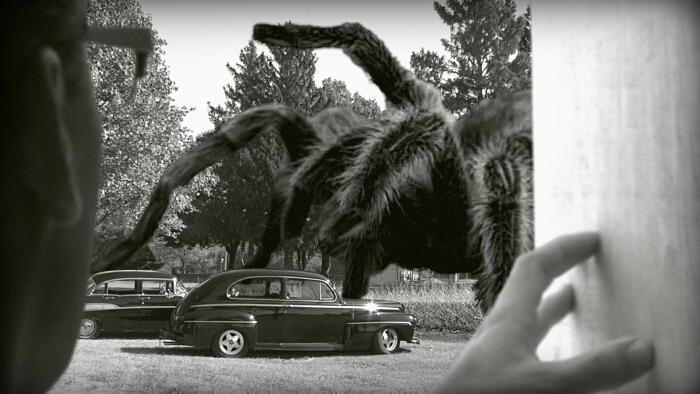
\includegraphics[height=4 cm]{Image25.jpg}
\clearpage
%-------------------------------------------------------
% slide ----------------------------------------------
\subsection{Some experimental results}
\footnotesize
\begin{flushleft}
A simple experiment:\\
(1) define a symbol generator as a 2-state Markov switching model\\
(2) use the switching model to simulate a time series data set (t=1000)\\
(3) use the empirical frequencies in the time series data to extract the conditional probabilities\\
(4) use the empirically-derived conditional probabilities to define the empirical, 1-step Markov chain\\
(5) compare the empirically-derived Markov chain to the Markov chain in the symbol generator\\
(6) repeat (1)-(5) with another symbol generator model\\
(7) try a bootstrap version
\end{flushleft}

\clearpage
%-------------------------------------------------------
% slide ----------------------------------------------
\subsection{Some experimental results}
\centering 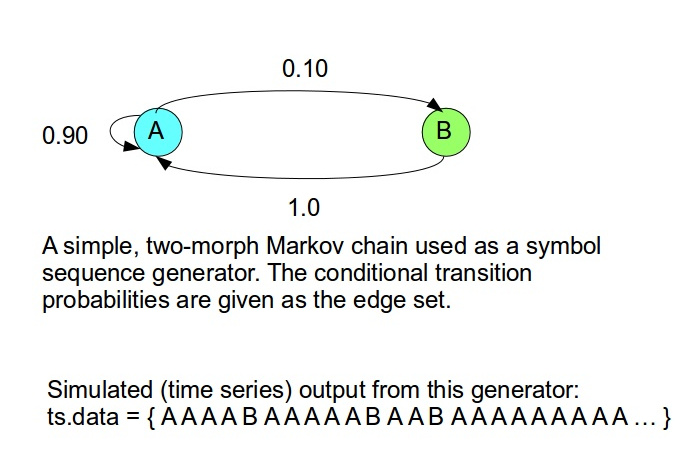
\includegraphics[height=5 cm]{Image26.jpg}

\clearpage
%-------------------------------------------------------
% slide ----------------------------------------------
\subsection{Some experimental results}
\tiny 
\begin{multicols}{2}
\begin{verbatim}
G1<-matrix(c(.9,.1,1,0), 2, byrow=TRUE)
G1
     [,1] [,2]
[1,]  0.9  0.1
[2,]  1.0  0.0

eigen(G1)
$values
[1]  1.0 -0.1

library(expm)
tiks <- 15
a <- matrix(0, 4, 1)
for (i in 2:tiks){
 a <- cbind(a, c(G1 %^% i))
 if(identical(round(a[,i],5), round(a[,i-1],5))) 
 {  break
  }
}
\end{verbatim}
\vfill
\columnbreak
\begin{verbatim}
a
     [,1] [,2]  [,3]   [,4]    [,5]     [,6]      [,7]
[1,]    0 0.91 0.909 0.9091 0.90909 0.909091 0.9090909
[2,]    0 0.90 0.910 0.9090 0.90910 0.909090 0.9090910
[3,]    0 0.09 0.091 0.0909 0.09091 0.090909 0.0909091
[4,]    0 0.10 0.090 0.0910 0.09090 0.090910 0.0909090

limit.matrix1 <- round(matrix(a[,7], 2, byrow=FALSE),3)
limit.matrix1
      [,1]  [,2]
[1,] 0.909 0.091
[2,] 0.909 0.091

stat.dist1 <- limit.matrix1[1,]
stat.dist1
[1] 0.909 0.091
\end{verbatim}
\end{multicols}
\clearpage
%-------------------------------------------------------
% slide ----------------------------------------------
\subsection{Some experimental results}
\tiny 
\begin{multicols}{2}
\begin{verbatim}
library(distr)
 #Experiment1; Generator1; Dist1
exp1gen1d1 <- DiscreteDistribution (supp = c(1, 2),
prob = c(0.9, 0.1))
 #Experiment1; Generator1; Dist2
exp1gen1d2 <- DiscreteDistribution (supp = c(1, 2),
prob = c(1, 0))	

set.seed(74)
tiks<-1000
Y_0<-1   #at t=0 ==> State 1
Y.G1.data <- NULL	#empty vector
Y.G1.data[1] <- Y_0

for (i in 2:tiks) {
 if (Y.G1.data[i-1]=="1"){
  Y.G1.data[i] <- r(exp1gen1d1)(1)
 }else if (Y.G1.data[i-1]=="2"){ 
  Y.G1.data[i] <- r(exp1gen1d2)(1)
 }
}
\end{verbatim}
\vfill
\columnbreak
\begin{verbatim}
Y.G1.data
 [1] 1 1 1 1 2 1 1 1 1 1 2 1 1 2 1 1 1 1 1 1 1 ...
 [39] 2 1 2 1 1 1 1 1 1 1 2 1 1 1 1 1 2 1 1 1 1 ...
 [77] 1 1 1 1 1 1 1 1 1 1 1 1 1 1 1 1 1 1 1 1 1 ...
[115] 2 1 1 1 1 1 1 1 1 1 1 1 1 1 1 1 1 1 1 1 1 ...
...................................................
[837] 1 1 1 1 1 1 1 1 1 1 1 2 1 1 1 1 1 1 1 1 2 ...
[875] 1 1 1 1 1 2 1 1 1 1 1 1 1 1 1 1 1 1 1 1 1 ...
[913] 1 1 1 1 1 1 1 1 1 1 1 1 1 1 1 1 1 1 1 1 1 ...
[951] 1 1 1 1 1 1 1 1 2 1 1 1 1 1 2 1 1 1 1 1 1 ...
[989] 1 1 1 2 1 1 1 1 1 2 1 1
\end{verbatim}
\end{multicols}

\clearpage
%------------------------------------------------------------
% slide ----------------------------------------------
\subsection{Some experimental results}
\tiny 
\begin{multicols}{2}
\begin{verbatim}
Y.G1.data.ts <- as.ts(Y.G1.data)
acf(Y.G1.data.ts, type = "correlation", 
main="Y.G1.data")

p.a <- sum(Y.G1.data=="1")/length(Y.G1.data)
[1] 0.906

p.b <- sum(Y.G1.data=="2")/length(Y.G1.data)
[1] 0.094

library(gtools)	
permutations(n=2,r=2,v=letters[1:2],
repeats.allowed=TRUE)
     [,1] [,2]
[1,] "a"  "a" 
[2,] "a"  "b" 
[3,] "b"  "a" 
[4,] "b"  "b"
\end{verbatim}
\vfill
\columnbreak
\begin{verbatim}
#automated counting window
count.bigrams <- NULL
for (i in 1:999) {
   #bi-gram {11} ==> "1"
if(identical(window(Y.G1.data.ts, i, i+1)[1:2], c(1,1))){
	count[i]<-1
	}else{
   #bi-gram {12} ==> "2"
if(identical(window(Y.G1.data.ts, i, i+1)[1:2], c(1,2))){
	count[i]<-2
	}else{
   #bi-gram {21} ==> "3"	
if(identical(window(Y.G1.data.ts, i, i+1)[1:2], c(2,1))){
	count[i]<-3
	}else{
   #bi-gram {22} ==> "4"
if(identical(window(Y.G1.data.ts, i, i+1)[1:2], c(2,2))){
	count[i]<-4
	}
      }
    }
  }
}
\end{verbatim}
\end{multicols}

\clearpage
%------------------------------------------------------------
% slide ----------------------------------------------
\subsection{Some experimental results}
\tiny 
\begin{multicols}{2}
\begin{verbatim}
table(count.bigrams)
count.bigrams
  1   2   3 
811  94  94 

p.aa <- 811/1000
p.ab <- 94/1000
p.ba <- 94/1000
p.bb <- 0/1000
---- results: Pr(a|a) ----------------
p.a_a <- p.aa/p.a
[1] 0.8962472
---- results: Pr(a|b) -------------------
p.a_b <- p.ba/p.b
[1] 1
---- results: Pr(b|a) --------------------
p.b_a <- p.ab/p.a
[1] 0.1037528
---- results: Pr(b|b) --------------------
p.b_b <- p.bb/p.b
[1] 0

\end{verbatim}
\vfill
\columnbreak
\begin{verbatim}
empirical.G1<-round(matrix(c(p.a_a, p.b_a, p.a_b, p.b_b), 
2, byrow=TRUE), 3)

empirical.G1
       [,1]  [,2]
[1,] 0.896 0.104
[2,] 1.000 0.000

library(expm)
tiks <- 15
b <- matrix(0, 4, 1)
for (i in 2:tiks){
  b <- cbind(b, c(empirical.G1 %^% i))
  if(identical(round(b[,i],5), round(b[,i-1],5))) {
    break
  }
}

emp.stat.dist1
[1] 0.906 0.094
\end{verbatim}
\end{multicols}

\clearpage
%------------------------------------------------------------
% slide ----------------------------------------------
\subsection{Some experimental results}
\tiny 
\begin{multicols}{2}
\begin{verbatim}
library(entropy)
   #5 different hypothesized stationary prob dists
   #d3 = the empirically-derived stationary distr
   #d_true = the known stationary distr
d1<- c(.99,.01)
d2<- c(.95,.05)
d3<- c(0.906, 0.094)  
d4<- c(.90,.10)
d5<-c(.85,.15)
d_true<- c(0.909, 0.091) 

		#as matrix
dM <- t(as.matrix(data.frame(d1,d2,d3,d4,d5)))
    [,1]  [,2]
d1 0.990 0.010
d2 0.950 0.050
d3 0.906 0.094
d4 0.900 0.100
d5 0.850 0.150

\end{verbatim}
\vfill
\columnbreak
\begin{verbatim}
  #calc KL divergence for each distr
  #place results in a matrix, KLM
KLM <- matrix(0, 5, 1)
for (i in 1:5){
	KLM[i,1] <- KL.empirical(d_true, dM[i,], unit="log2")
}

KLM
            [,1]
[1,] 1.779721e-01
[2,] 2.076308e-02
[3,] 7.696969e-05  #closest to known stationary distr
[4,] 6.673603e-04
[5,] 2.239388e-02

\end{verbatim}
\end{multicols}

\clearpage
%------------------------------------------------------------
% slide ----------------------------------------------
\subsection{Some experimental results}
\tiny 
\begin{multicols}{2}
\begin{verbatim}
#bootstrap for a (small) time series data set
(t=51)
Y.G1.data
 [1] 1 1 1 1 2 1 1 1 1 1 2 1 1 2 1 1 1 1 1 ...
 [39] 2 1 2 1 1 1 1 1 1 1 2 1 1 1 1 1 2 1 1 ...
 [77] 1 1 1 1 1 1 1 1 1 1 1 1 1 1 1 1 1 1 1 ...
[115] 2 1 1 1 1 1 1 1 1 1 1 1 1 1 1 1 1 1 1 ...
................................................
[951] 1 1 1 1 1 1 1 1 2 1 1 1 1 1 2 1 1 1 1 ...
[989] 1 1 1 2 1 1 1 1 1 2 1 1

sampled.output.G1 <-as.ts(Y.G1.data[250:300])
\end{verbatim}
\vfill
\columnbreak
\begin{verbatim}
stat1 <- function(tsb){
count <- NULL
for (i in 1:50) {
if(identical(window(tsb, i, i+1)[1:2], c(1,1))){
  count[i]<-1
  }else{
if(identical(window(tsb, i, i+1)[1:2], c(1,2))){
  count[i]<-2
  }else{
if(identical(window(tsb, i, i+1)[1:2], c(2,1))){
  count[i]<-3
  }else{
if(identical(window(tsb, i, i+1)[1:2], c(2,2))){
  count[i]<-4
	}
      }
    }
  }
}
	a <- c(sum(tsb=="1"), sum(tsb=="2"))
	b<-table(count)
	c(a[1], a[2], b[1], b[2], b[3], b[4])
}
\end{verbatim}
\end{multicols}

\clearpage
%------------------------------------------------------------
% slide ----------------------------------------------
\subsection{Some experimental results}
\tiny 
\begin{multicols}{2}
\begin{verbatim}
library (boot)
set.seed <- 477
boot1<-tsboot(sampled.output.G1, stat1, 1000, 5, 
"geom")

boot1$t[is.na(boot1$t)]<-0
bs.means <- colMeans(boot1$t[,1:6])
[1] 46.994  4.006 42.212  3.860  3.865  0.063

(bs.p.a <- bs.means[1]/50)
(bs.p.b <- bs.means[2]/50)

(bs.p.aa <- bs.means[3]/50)
(bs.p.ab <- bs.means[4]/50)
(bs.p.ba <- bs.means[5]/50)
(bs.p.bb <- bs.means[6]/50)

bootstrap.G1
         [,1]       [,2]
[1,] 0.9080521 0.09194791
[2,] 0.9745382 0.02546181
\end{verbatim}
\vfill
\columnbreak
\begin{verbatim}
#convergence after 7 iterations
btstrp.stat.dist1
[1] 0.914 0.086

  #KL for 5 different hypothesized stat. prob. dists
  #[3,]=the bootstrap-derived stationary dist
            [,1]
[1,] 0.1779721139
[2,] 0.0207630769
[3,] 0.0002255110	#still the closest to the known distr
[4,] 0.0006673603
[5,] 0.0223938764

#compare KL values
KL for empirically-derived stationary distr
0.000077 = 77 x 10^-6 

KL for bootstrap-derived stationary distr
0.000230 = 230 x 10^-6
\end{verbatim}
Not bad! (KL = 0 implies identical prob dist.s)
\end{multicols}

\clearpage
%------------------------------------------------------------
% slide ----------------------------------------------
\section{Lots to do!}
\subsection{Pitfalls and challenges}
\small
\begin{flushleft}
* defining state variables that capture multiple scale dynamics\\
* defining phase space partitions\\
* defining the landscape reference scenarios\\
* ag in LANDIS-II\\
* dangers of using Markov chains \\
* the ingression of novelty
\end{flushleft}

\clearpage
%------------------------------------------------------------
% slide ----------------------------------------------
\section{Lots to do!}
\subsection{Next steps}
\small
\begin{flushleft}
* evaluate state variables\\
* evaluate ag in LANDIS-II\\
* run tests with 'dummy' landscapes
\end{flushleft}

\clearpage
%------------------------------------------------------------
% slide ----------------------------------------------
\section{That's it folks!}
\subsection{Thanks.}
\centering 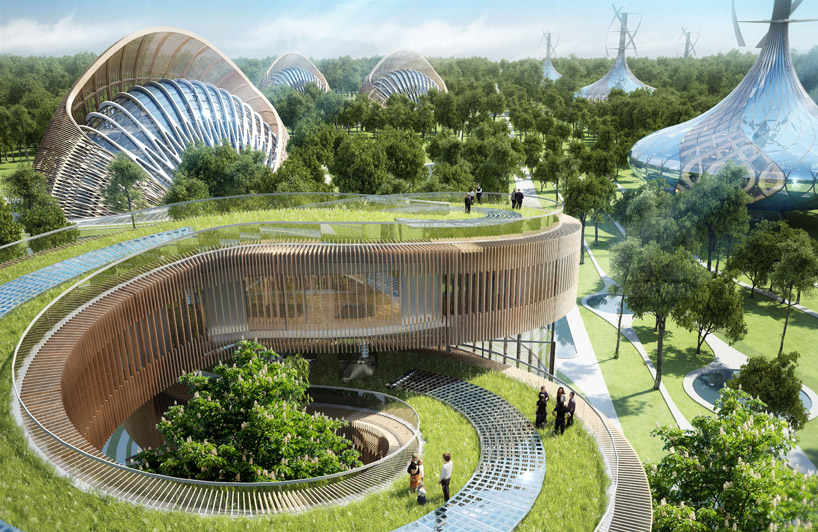
\includegraphics[height=5 cm]{Image27.jpg}
Vincent's orchard
\clearpage
%------------------------------------------------------------

\end{document}
